
%%%%%%%%%%%%%%%%%%%%%%%%%%%%%%%%%%%%%%%%
%\documentclass[review]{cje}
% \documentclass[proof]{cje}
\documentclass{cje}
%%%%%%%%%%%%%%%%%%%%%%%%%%%%%%%%%%%%%%%%

% Package for bibliography in CJE format. 
\usepackage{cjenatbib}

% For displaying urls within text.
\usepackage{url}

% For rendering eps figures to pdf on different platforms. 
\ifx\pdftexversion\undefined
    \usepackage[dvips]{graphicx}
\else
    \usepackage[pdftex]{graphicx}
    \usepackage{epstopdf}
    \epstopdfsetup{suffix=}
\fi

% Mathematical notation. 
\usepackage{amssymb,amsmath,amsthm}

% Just for bold Greek letters in equations.
\usepackage{bm}

% For separate horizontal lines in LPM vs Logit tables.
\usepackage{booktabs}

% Reduce spacing between coulmns in LPM vs Logit tables.
\setlength{\tabcolsep}{2.5pt}

%%%%%%%%%%%%%%%%%%%%%%%%%%%%%%%%%%%%%%%%
\begin{document}
\label{firstpage}
%%%%%%%%%%%%%%%%%%%%%%%%%%%%%%%%%%%%%%%%

\title[Penalties for Speeding and their Effect on Moving Violations]{Penalties for Speeding and their Effect on Moving Violations: Evidence from Quebec Drivers}

\authors{V.~Chandler, L.~Morin, J.~Penney} 

\authorone{Vincent Chandler}{Universit\'{e} du Qu\'{e}bec en Outaouais}

\authortwo{Lealand Morin}{University of Central Florida} 

\authorthree{Jeffrey Penney}{University of Alberta} 

\JEL{K42, K49}

\acknowledgements{The authors would like to thank 
Fran\c{c}ois Tardif for his help with the data in the early stages of this project, 
as well as  
Catherine Maclean 
for helpful suggestions and valuable comments. 
Jeffrey Penney acknowledges support from SSHRC. 
The authors are especially grateful to the editor and two anonymous referees 
for comments and suggestions that led to substantial improvements from the original manuscript. 
The authors have no conflict of interest to disclose. 
The usual caveat applies.}

%%%%%%%%%%%%%%%%%%%%%%%%%%%%%%%%%%%%%%%%

\abstract{

	In 2008, the province of Quebec drastically increased penalties for speeding 
	well above the speed limit by doubling fines and instituting on-the-spot licence suspension. 
	Using administrative driving and licensing records in Quebec from 2006 to 2010, 
	we examine whether the new law discouraged unlawful driving behaviour 
	by investigating the frequency with which motorists received traffic citations. 
	We find that the new law was effective in deterring motorists from speeding.
	Moreover, the effect was most pronounced for males compared to females, 
	for young compared to old, 
	and especially so for drivers with high demerit point balances accumulated from past
	infractions compared to those with few or no tickets. 
	In sum, the change in behaviour was most apparent for 
	those drivers who were the intended targets for the legislation. 
	
	
	\medskip
	\noindent
	Keywords: driving behaviour, law enforcement, risk aversion, speeding.


         }

%\resume{
%
%        \input{Text/Resume}
%
%       }

%%%%%%%%%%%%%%%%%%%%%%%%%%%%%%%%%%%%%%%%

\maketitle

%%%%%%%%%%%%%%%%%%%%%%%%%%%%%%%%%%%%%%%%

\section{Introduction}
\label{sec:Introduction}

In 2018, 1,743 individuals died in Canada following a car accident 
\citep{transcan2018}. 
Such accidents are the leading cause of death for individuals aged between 15 and 44
\citep{statscan2020}.   
Many OECD countries have recently introduced harsher punishments to deter 
the types of behaviour that increase the likelihood of such tragedies. 
For example, penalties for speeding well above the speed limit now typically include 
some combination of substantially increased fines, immediate vehicle seizure, and licence suspension.
These laws are typically referred to as excessive speeding laws or stunt driving laws. 

Quebec followed this trend and introduced excessive speeding penalties in 2008. 
Its provisions are triggered when driving well above the speed limit. 
For example, driving at a speed of 100km/h in a 60km/h zone would be considered excessive speeding.
These harsher punishments received widespread media coverage 
both before and after the change in legislation, 
and there was a sustained campaign by the provincial government 
to help ensure drivers were aware of the law. 
The Quebec government has since declared the legislation to be successful, 
with the number of excessive speeding tickets decreasing over time.%
\footnote{The legislation has been unsuccessfully challenged in court.}
%
Furthermore, the number of accidents resulting in bodily harm 
decreased from 36,816 in 2006 to 32,371 in 2010, 
and the number of fatal accidents decreased from 666 to 441 
over the same period 
\citep{saaq2011}. 
Even though these findings are encouraging, 
they don’t provide conclusive evidence that the harsher penalties truly caused changes in driving behaviour. 


Since 
\citet{becker1968b}, 
economists have theorized that harsher punishments 
alter the incentives of individuals and thus ultimately their behaviour. 
\citet{hellandtabarrok2007} 
provide evidence for this mechanism 
studying the impact of California’s three-strike legislation on the recidivism rates of felons. 
However, the effectiveness of deterrence is unclear in the context of driving. 
Indeed, 
\citet{bourgeonpicard2007} 
hypothesize that some drivers may be impossible to deter 
either because they do not care about the penalties or because they are not aware they are speeding.


A broad literature has investigated the role of deterrence on driving 
and particularly alcohol consumption 
\citep[e.g.][]{hansen2015}, 
but less attention has been devoted to speeding. 
Some empirical research has determined the impact of very influential policies 
like the introduction of a demerit point system. 
For example, 
\citet{bennedittiniNicita2009} 
show a reduction in road fatalities 
through deterrence and incapacitation following the introduction of such a system. 
More generally, 
\citet{castillocastro2012} 
provide a meta-study 
demonstrating the broad positive impact of such a policy in a variety of countries. 
In Quebec, 
\citet{dionneetal2011} 
focus on the threat of the loss of licence 
on the behaviour of a driver close to the demerit point threshold of suspension. 
They find a reduction in the probability of violation for drivers 
with a large number of demerit points and conclude 
the system is successful in deterring the worst offenders. 
Finally, closest to this paper, 
\citet{meirambayeva2014} 
show the introduction of a street-racing law in Ontario decreased the number of accidents 
by conducting an intervention analysis with an ARIMA model of 
the monthly number of accidents in Ontario.
%
Using monthly, aggregated data, 
they find an intervention effect for young males
but not for females or mature males. 


In this paper, we investigate the effect of Quebec’s excessive speeding legislation
on the frequency and types of violations incurred by Quebec drivers 
using an event-study design. 
Such violations are a proxy for driving behaviour, 
so this study will glean insight into the effect of increasing penalties on dangerous driving. 
It is important to note that we are looking at all violations which result in demerit points, 
and not just those that are affected by the change in the law. 
% 
In contrast to \citet{meirambayeva2014}, 
our focus on traffic violations
studies an event further up the chain of causation that happens more frequently. 
Although these events are still rare,
we can measure gender and age differences more precisely, 
using a very large dataset of individual drivers with daily observations. 

We analyze driving records obtained from administrative data sets 
of the Government of Quebec comprising the universe of violations 
from 2006 to 2010 and records on driver's licences over the same period. 
The use of large administrative datasets is necessary because only a small fraction 
of all drivers are impacted by the policy change; 
yet, these drivers are particularly important because they are 
generally responsible for accidents causing bodily harm and property damage. 
% 
We first present a simple theoretical model to examine the predictions of economic theory 
on the effect of the law on drivers.
%
It predicts heterogeneous effects by age and gender,  
which guides our regression analysis. 
% 
We then examine the heterogeneous effects of the excessive speeding law 
on both the extensive margin (getting a ticket) 
and the intensive margin (getting a more severe ticket) across gender and age. 


We find that the daily probability of receiving a ticket (extensive margin) 
decreases after the implementation of the law. We first focus our attention on the impact of the policy for different age groups and genders.
Young drivers between the ages of 16 and 24 are the most affected by the law, 
while there is little effect for drivers over the age of 45. 
Even though both males and females change their behaviour, the magnitude of the effect on males is about eight times the effect on females. 
We then consider the effect of the policy on drivers who have a history of speeding. First, we assess the impact of the policy on drivers who had between 6 and 10 points on a given day. The effect of the policy is five times larger for this group relative to the average driver. Second, we focus our attention on drivers who have had between 6 and 10 points in the pre-sample period and find similar results. Finally, we show that male drivers with more demerit points react more strongly to the policy.

We then investigate the effect on the intensive margin, which we define as the point value of the tickets when they occur. 
For males, the probability of getting tickets worth only one demerit point 
actually increases following the new policy, while tickets for all other point values decrease. 
This result suggests that male drivers are still exceeding the speed limit 
but are driving more slowly than before the introduction of the legislation. 
A similar pattern exists for female drivers for one and two point violations. 
%
We conclude that Quebec’s 2008 excessive speeding law has had substantial spillover effects 
on both the extensive and intensive margins of driving behaviour. 
In other words, not only has the policy reduced the number of drivers driving well above the speed limit, 
it has also led to a decrease in the propensity to commit other moving violations.
% 
More importantly, although the effect is noticed for average drivers, 
who are mainly not speeding, 
we observe a substantial response from the drivers who are generally more likely to get tickets%
---those who are appropriate targets for the legislation. 

This paper contributes to the literature in several ways. 
It is the first examination using administrative data into the effect of 
an excessive speeding law on driving behaviour 
as proxied by violations by gender and age group. 
Such analysis is important because most countries currently use demerit point systems. 
The question now is not whether these systems work 
but whether and how they can be adjusted to increase road safety. 
Moreover, this paper is to our knowledge the first one to empirically investigate 
the impact of such laws on both the intensive and extensive margins of speeding. 
Finally, by studying the impact of deterrence by gender and age, 
this paper helps to fill a gap acknowledged by 
\citet{freeman1999}
on the role of gender in studies surrounding criminality.


The rest of this article is organized as follows. 
Section \ref{sec:Background} covers the details of Quebec’s excessive speeding law 
and the relevant institutional background. 
The data and summary statistics are presented in Section \ref{sec:Data}. 
% 
We construct a simple theoretical model investigating the effects of the law
that forms the basis of our empirical specification in Section \ref{sec:Model}. 
% 
In Section \ref{sec:Empirical}, we conduct the empirical analysis. 
Robustness checks and placebo regressions are conducted in Section \ref{sec:Validity}. 
We conclude with a policy discussion in Section \ref{sec:Discussion}.



%%%%%%%%%%%%%%%%%%%%%%%%%%%%%%%%%%%%%%%%

\section{Institutional background}
\label{sec:Background}

Vehicular conveyance in the province of Quebec is primarily overseen by 
a public organization known as the Soci\'{e}t\'{e} de l'assurance automobile du Qu\'{e}bec, 
commonly abbreviated as SAAQ. 
This organization was legislated into existence in 1978 and has several mandates. 
First, it has a public monopoly on the portion of insurance that covers bodily injury. 
Second, it is responsible for enforcing two key pieces of legislation relating to driving: 
the Highway Safety Code and the Automobile Insurance Act.\footnote{%
%
A current list of offences that result in demerit points under the Highway Safety Code 
can be found at the following web address: 
\url{https://saaq.gouv.qc.ca/en/drivers-licences/demerit-points/offences-and-demerit-points/} (Accessed May 29, 2020).}
%
Finally, it manages the driving records of Quebec drivers, 
including the demerit point system, 
and the organization promotes road safety through awareness campaigns.

The demerit point system generally operates along the following lines. 
If a driver is caught committing a violation, the police officer 
gives the person a ticket according to the violation in question. 
All violations include a fine and a number of demerit points. 
Drivers can either admit guilt by paying the ticket or challenge the sanction in court. 
The violation is recorded in the driver’s file when the guilty plea is received 
or when the judge convicts the driver. 
The points are added to the driver’s file when the violation is recorded 
and remain there for a period of 24 months. 
If drivers accumulate points beyond a particular threshold, 
they lose their licence for a period of time 
after which they can reapply for one.\footnote{%
%
The threshold depends on the driver's age and type of driver’s licence 
(e.g., learner’s permit)
and the term of the licence suspension 
increases every time drivers lose their licence.}
%
They will only receive a new licence if they successfully complete 
the theoretical and practical driving examinations.



\begin{table}% [ht]
\centering
\begin{tabular}{p{1.5cm} p{1.5cm} p{2cm} p{2.5cm} p{2.5cm}}
  \hline
     				& First  	& Second	& Third 	& Subsequent  \\ 
				& offence	& offence	& offence 	& offences \\
  \hline
Licence suspension
	&  7 days
		& 30 days
			& 60 days if all three offences were committed in a zone of 60km/h or less, 
				otherwise 30 days
				& 60 days if this offence and at least two others were committed 
					in a zone of 60km/h or less, otherwise 30 days \\
   \hline
Vehicle seizure 
	& none
		& 30 days if both offences committed in a zone of 60km/h or less
			& 30 days if this offence and at least one other were committed 
				in a zone of 60km/h or less
				& 30 days if this offence and at least one other were committed 
					in a zone of 60km/h or less \\
   \hline
Fines			& doubled			& doubled			& doubled			& doubled \\
   \hline
Demerit Points	& doubled			& doubled			& doubled			& tripled \\
   \hline
\end{tabular}
\caption{Penalties for Excessive Speeding} 
\label{tab:penalties}
\end{table}

Quebec’s excessive speeding law came into force on April 1, 2008 
and changed the demerit point system managed by the SAAQ.\footnote{%
%
On September 30, 2007, the Ontario government introduced legislation against street racing. 
If drivers decided to go to Quebec to engage in street racing to avoid this law, 
these tickets would not be in this database, 
because these drivers would not have a Quebec driver's licence.} 
% 
This change was advertised by the SAAQ both before and after the law came into effect. 
Excessive speeding is defined by the law as exceeding the speed limit 
by 40 km/h in a zone of 60 km/h or less, 
by 50 km/h in a zone between 60 to 90 km/h, 
and by 60 km/h in a zone where the speed limit is equal to or greater than 100 km/h. 
The law worked in tandem with the then currently legislated speeding violations, 
increasing fines and demerit point penalties 
and imposing licence suspensions and vehicle seizures. 
Although offences involving demerit points remain on a person’s driving record for two years,
excessive speeding convictions remain on a person’s driving record for 10 years. 
% 
Table \ref{tab:penalties} details the penalties for violating the excessive speeding law. 
Note that the licence suspension and vehicle seizure occur 
immediately after being pulled over regardless of the driver’s innocence or guilt, 
while the fines and demerit points are only entered into the record 
once the individual admits guilt or is later found guilty in a court of law. 


%%%%%%%%%%%%%%%%%%%%%%%%%%%%%%%%%%%%%%%%

\section{Data}
\label{sec:Data}


We use records of traffic violations and drivers licences obtained 
from SAAQ administrative data to generate a dataset containing 
the universe of driver-days from April 1, 2006 to March 31, 2010 
for the province of Quebec.\footnote{%
The dataset on driver’s licences allows us to include observations 
that do not receive any tickets during the sample period.}  
Our dataset contains information on the age, gender, 
and details concerning traffic violations of the offender. 
In all, we have approximately 9.7 billion driver-day observations 
over the sample period. 
This very large sample will afford us the opportunity to examine 
detailed subgroups and give us the statistical power 
to detect effects that are small in absolute magnitude.

We begin with a graphical examination of monthly ticket frequencies for given point values 
before and after the policy change. 
%
Unfortunately, the dataset does not distinguish directly 
between single and multiple violations for a single police stop. 
For example, a driver with two 3-point violations 
is recorded the same as 
a driver with a single 6-point violation---all we observe is that 
both drivers gained 6 demerit points on a given day. 
In some cases, however, we can deduce from the demerit point values 
that multiple violations occurred, because there is no single violation with this particular number of points.
%
Fortunately, multiple violation stops are likely very rare in our sample.%
\footnote{%
For example, before the excessive speeding law, 
there were no violations worth 6 points, 
but the sample shows 517 stops resulting in 6 demerit points 
compared to 43,006 stops resulting in 5 demerit points. 
As another example, a single 7-point violation was present 
before the policy change, but none after; 
the number of 7-point tickets before the policy change was 8,366, 
and it decreased to only 24 after the policy change. 
There are no violations in the Highway Safety Code worth 8 or 11 demerit points 
at any time in our sample period, 
and our data shows no stops with demerit point totals of these values.}

Since the demerit point values of some violations doubled 
after the excessive speeding law came into effect, 
% 
we will compare stops associated with a certain number of points 
before the policy change with those associated with the 
same number of points and double the number of points after the policy change. 
For example, a driver speeding 46km/h to 49km/h over the speed limit 
before the policy change would receive a 5-point ticket, 
but the same violation would be worth 10 points after the policy change 
if it qualifies for excessive speeding. 
Because excessive speeding doubles the point values of some speeding violations, 
we will need to compare the frequency of 5-point stops before the policy change 
to 5- or 10-point stops afterwards 
(as not all 5-point speeding violations may qualify as excessive speeding). 
Due to the aforementioned possibility of stops with multiple violations, 
the number of tickets with 5- or 10-point values may contain 
combinations of violations which will be counted in the post period 
that were not counted in the pre period. The effect of the law 
will thus be underestimated in this case, even though this effect should be minimal.

If drivers do not adjust their behaviour, 
there should be about as many drivers with 5 points before the policy 
as there were drivers with 5 or 10 points after the policy. 
If drivers slow down, the number of 5-point or 10-point violations will decrease. 


\begin{figure}
\centering
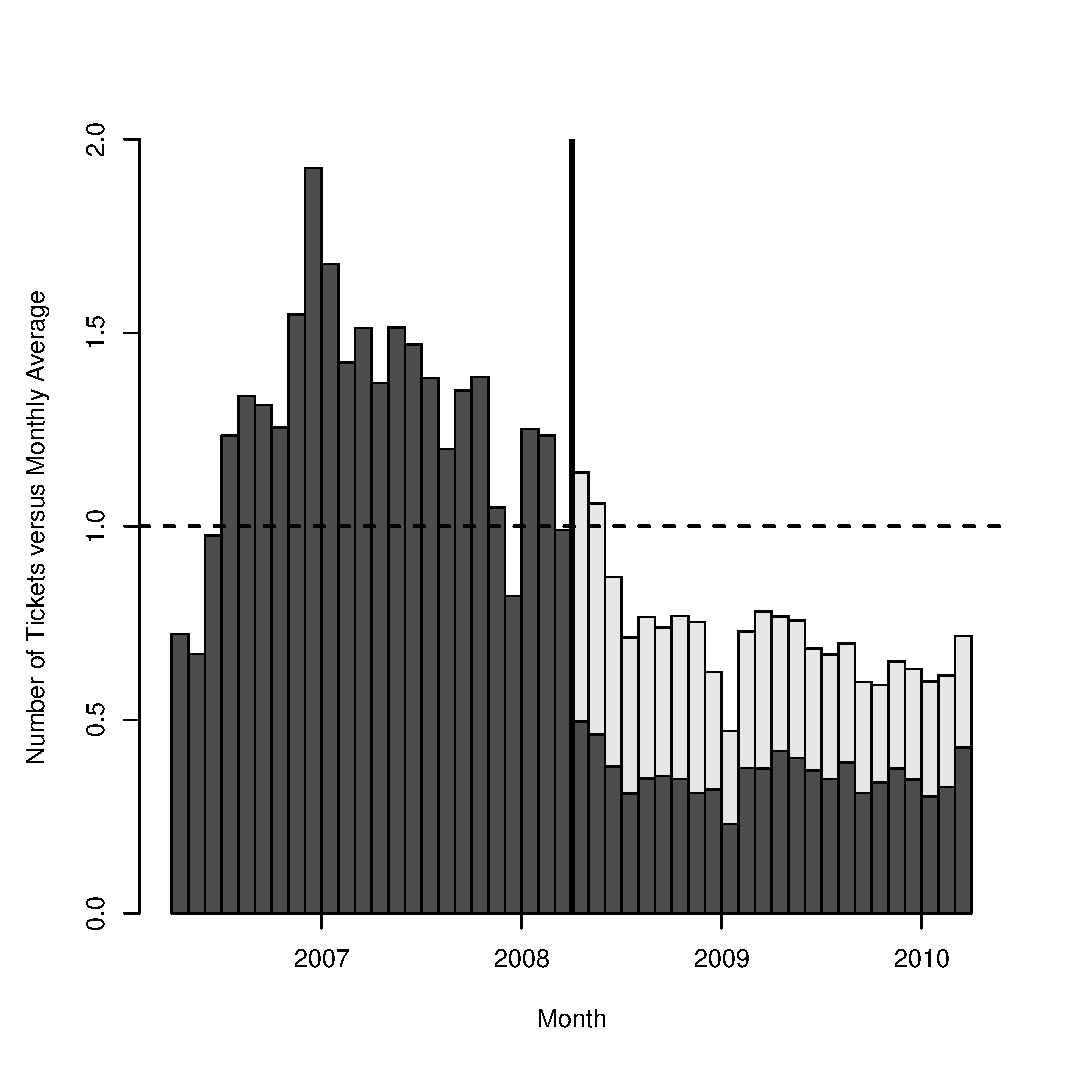
\includegraphics[width=0.8\textwidth]{Figure1}
\caption{Monthly frequency of 5- and 10-point violations \\
Monthly frequency of 5-point violations are shown before the policy change 
and 5- or 10-point violations are shown after, 
divided by the average number of 5- and 10-point violations
for each calendar month. 
% 
The dashed line at $1.0$ indicates the point at which 
the number of tickets is equal to the average for each month 
for tickets of the same point values over the entire sample.
% 
Dark grey areas correspond to 5 point-stops and light grey areas to 10-point stops.
}\label{fig:num_pts_5_10_all}
\end{figure}


Taking into consideration the seasonality of speeding, we see 
in Figure \ref{fig:num_pts_5_10_all}
an important reduction in the number of 5- or 10-point tickets 
in the summer of 2008 compared to the preceding summer. 
Overall, there is a general downward trend in the number of tickets 
after the policy change compared to before the policy change, 
and the 5- and 10-point tickets after the change are approximately evenly split. 

Figure \ref{fig:num_pts_7_14_all} focuses our attention on 7- or 14-point tickets. 
Nearly all 7-point violations are worth 14 points after the policy change, 
while only a few 7-point violations remain. 
Since there is no violation worth 7 points after the policy change, 
all of the 7-point stops after the policy change are due to being pulled over 
for multiple violations totalling 7 points. 
Once again, we see a downward trend in the number of total violations. 


\begin{figure}
\centering
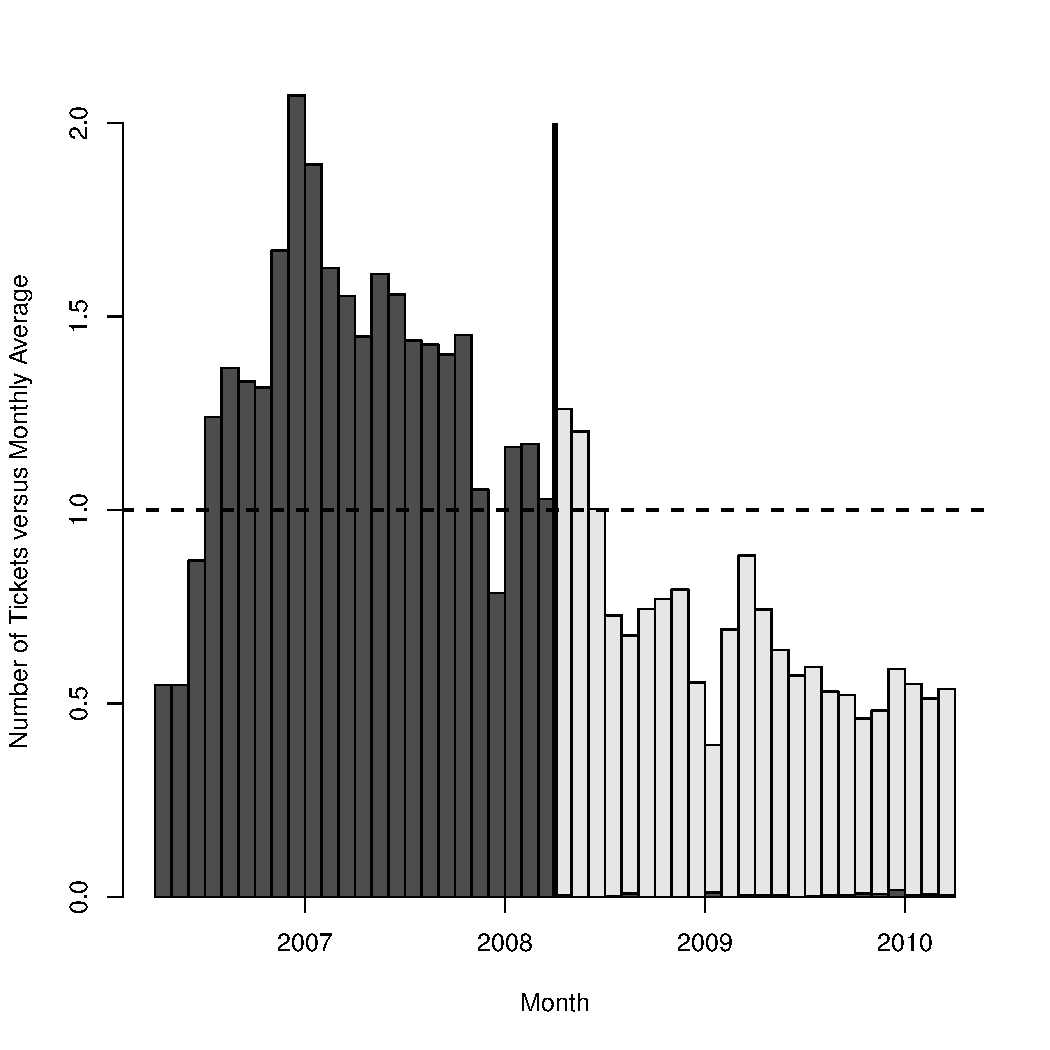
\includegraphics[width=0.8\textwidth]{Figure2}
\caption{Monthly frequency of 7- and 14-point violations \\
Monthly frequency of 7-point violations are shown before the policy change 
and 7- or 14-point violations are shown after, 
divided by the average number of 7- and 14-point violations
for each calendar month. 
% 
The dashed line at $1.0$ indicates the point at which 
the number of tickets is equal to the average for each month 
for tickets of the same point values over the entire sample.
% 
Dark grey areas correspond to 7 point-stops and light grey areas to 14-point stops.
}\label{fig:num_pts_7_14_all}
\end{figure}



\begin{table}% [ht]
\centering
\begin{tabular}{r r r r r r r}
  \hline
		& \multicolumn{2}{c}{Male Drivers} 	&  \multicolumn{2}{c}{Female Drivers} &  \multicolumn{2}{c}{Gender Ratio} \\
 & & & & & \multicolumn{2}{c}{(Percent Males)} \\

 \cmidrule(lr){2-3}\cmidrule(lr){4-5}\cmidrule(lr){6-7} 
%  \hline
Points 	& Pre 		& Post		& Pre 		& Post		& Pre 		& Post		\\ 
  \hline
1 		& 101,298 	& 122,899	&  45,382 	&   61,778 	& 69\% 	& 67\% \\ 
2 		& 533,167 	& 572,194	& 249,669 	& 283,108 	& 68\% 	& 67\% \\ 
3 		& 701,053 	& 627,807	& 247,991	& 239,554	& 74\% 	& 72\% \\ 
4 		&  15,567 	&  15,278 	&    2,216 	&    2,470 	& 88\% 	& 86\% \\ 
5 		&  43,006 	&  12,368 	&    8,172 	&    2,272 	& 84\% 	& 84\% \\ 
6 		&     496 	&  12,000 	&        21 	&    3,296 	& 96\% 	& 78\% \\ 
7 		&   7,688 	&        18 	&      648 	&          6 	& 92\% 	& 75\% \\ 
9 		&   7,382 	&    5,791 	&    2,587 	&    2,431 	& 74\% 	& 70\% \\ 
10 		&         0 	&  12,747 	&         0 	&    2,137 	& -			& 86\% \\ 
12 		&     127	&         0 	&         1 	&         0 	& 99\% 	& - \\ 
14 		&       0 	&   4,145 	&         0 	&      302 	& -			& 93\% \\ 
15 		&      17 	&         0 	&         1 	&         0 	& 94\% 	& - \\ 
18 		&       3 	&      560 	&         0 	&        23 	& 100\% 	& 96\% \\ 
24 		&       0 	&       98 	&         0 	&         4 	& -			& 96\% \\ 
30 		&       0 	&       17 	&         0 	&         0 	& -			& 100\% \\ 
36 		&       0 	&        4 	&         0 	&         0 	& -			& 100\% \\ 

   \hline

Total 	  & 1,409,804 & 1,385,926 & 556,688 & 597,381 & 72 & 70 \\ 

   \hline
\end{tabular}
\caption{Frequency of tickets by point value} 
The ``Pre'' and ``Post'' columns refer to offences that occurred before and after the policy change, which occurred on April 1, 2008. 
Our sample covers the four-year window from April 1, 2006 to March 31, 2010, 
leaving a symmetric window of two years for each of the ``Pre'' and ``Post'' policy periods.
The gender ratio is measured as the percentage of the number of offences committed by males 
divided by the total number of offences committed by all drivers. 
\label{tab:point_freq}
\end{table}

Table \ref{tab:point_freq} reports 
the number of tickets by point value, 
for male and female drivers, before and after the
change in penalties. 
%
In the 1- and 2-point categories, the number of tickets increases 
for both males and females on a per driver-day basis, 
and generally decreases in the higher-point categories. 
% 
Recall that several types of violations
earn a higher number of points after the policy change; 
for example, 
the 14-point tickets are all formerly 7-point tickets.

Before the excessive speeding law came into effect, 
the average driver had a probability of 0.04\% to receive a ticket 
on any particular day. This probability decreased by approximately 3.6\% after the policy change.
To put these numbers in a broader context, 
the vast majority of the sample are non-events. 

If we change our focus and look at the demerit points per driver per day, 
they decreased after the policy change for males by 6\% and by 1\% for females. 
This result is particularly interesting, 
because excessive speeding penalties doubled the value of many 
speeding violations previously worth 5, 7, and 9 points.\footnote{%  
Some 3-point speeding tickets are subject to the excessive speeding law, 
but the circumstances are quite particular: 
the suspect needs to be exceeding the speed limit in a zone 
with a posted limit of 60km/h or less by 40 to 45 km/h.}
In the absence of a change in behaviour, 
the number of demerit points per driver per day 
would have mechanically increased. 


Table \ref{tab:point_freq} also provides information on the distribution of both genders. Overall, females represent approximately half of all drivers 
yet only 20\% of all traffic tickets. 
%
The last two columns of the table
report the gender ratio by point value.
% 
Females claim one third of the tickets for 1 or 2 points
but only a quarter of 3-point tickets. 
Males account for the majority of tickets with higher point values, 
with the gender ratio approaching 100\% male 
for the most severe cases. 
% 
The extreme gender ratio in the upper tail suggests that males engage in risky driving behaviour 
more often than females. 

%

% 
Economists
\citet{crosongneezy2009}
document a large literature 
analyzing gender differences in preferences from many perspectives, 
including financial decisions, as in
\citet{charnessgneezy2012}.   
% 
This topic has a long history in the psychological literature: 
\citet{byrnes1999}
reviewed
over 150 papers on gender differences in risk perception.
In their words, the literature ``clearly'' indicated that
``male participants are more likely to take risks than female
participants'' (p. 377). 
% 
Exploring factors aside from risk aversion, 
\citet{powellansic1997} report that the gender difference in risk-taking 
is irrespective of familiarity and framing, costs, or ambiguity. 
% 
\citet{harris2006} 
consider not only the incidence and severity of
negative outcomes but also the enjoyment expected from 
engaging in risky activities. 
This 
partially mediated the perceived lower propensity of females
toward risky choices in decisions involving gambling, recreation, and health. 
We explore these differences in perception to explain 
the differences in both 
the tendency for speeding and 
the reaction when the cost of speeding increases. 


Aside from gender differences, 
there also exists the potential for differences by age, 
which is also observed in our dataset. 
%
In fact, this is also one of the main findings in 
\citet{byrnes1999}: 
there were significant shifts in the size of the gender gap between successive age levels.
% 
We explore this further with a more precise empirical specification. 


%%%%%%%%%%%%%%%%%%%%%%%%%%%%%%%%%%%%%%%%

\section{Model}
\label{sec:Model}

In this section, we present a simple theoretical model of driving behaviour, 
%
which guides our empirical specification. 
%
We use this to appeal to economic theory to determine whether to expect 
differences in age and gender as a result of a policy that increases the risk of driving, 
and if so, whether there would be a pattern in these differences. 
% 
For simplicity, we focus on the two-dimensional comparison 
of risk preferences by gender. 
% 
We later use the conclusions reached from this analysis 
to provide testable predictions for the empirical analysis
of the population of drivers who differ by gender, age, 
and their historical records of traffic offences.  

Consider the utility maximization problem 
for the representative agent
%
% \begin{equation}
$$
	u_j (s) = g(s) - r_j (s)
$$
% \end{equation}
% 
where $g(s)$ is the utility of driving at speed $s$ 
and $r_j (s)$ is the disutility from the risk of driving at speed $s$, 
and $j$ indexes males and females $\{m,f\}$;
% 
therefore, we assume the representative male and the representative female 
have different risk preferences (and therefore utility functions). 
% 
Assume $g(s)$ is concave increasing $(g^{\prime} (s)>0, 
g^{\prime\prime} (s)<0)$ 
and $r_j (s)$ is convex increasing $(r_j^{\prime} (s)>0, r_j^{\prime\prime} (s)>0)$. 
Let $g(s)$ and $r_j (s)$ be continuous in the positive orthant. 
Impose the regularity conditions $g(s)\geq0 \forall s$ and $r_j (s)\geq0 \forall s$. 
Let there exist values of s such that $g(s)>r_j (s)>0$; 
this guarantees the existence of a non-trivial equilibrium. 
Taking the first order condition of the objective function, 
the ideal speed $s^*$ is chosen such that $g^{\prime} (s^*)=r_j^{\prime} (s^*)$, 
and this is a global maximum because 
$u_j^{\prime\prime} (s)=g^{\prime\prime} (s)-r_j^{\prime\prime} (s)<0$. 
Plotting each curve separately on a graph, 
the point $s^*$ maximizes the vertical distance between the concave and convex curves,
% 
and this occurs at the point where the slopes are equal. 
Let $r_m (s)<r_f (s)  \forall s$; 
that is, the perceived risk of driving at any given speed 
is higher for females than it is for males, 
following 
\citet{harris2006}
and consistent with
\citet{crosongneezy2009}.
Graphically, the risk function for the representative females will be more convex than it is for the representative male. 
Examining the first order conditions, 
we see that, on average, males will drive faster than females ($s_m^*>s_f^*$) 
since 
$u_m^{\prime} (s)
=g^{\prime} (s)-r_m^{\prime} (s)
>g^{\prime} (s)-r_f^{\prime} (s)
=u_f^{\prime} (s)$. \\


\textbf{Proposition 1.} {\it 
Let $u_j (s) = g(s) - r_j (s)$ represent consumers' utility, 
where $g(s)$ is the utility of driving at speed $s$ 
and $r_j (s)$ is the disutility from the risk of driving at speed $s$, 
both of which are continuous in the positive orthant. 
%
Assume $g(s)$ is concave increasing $(g^{\prime} (s)>0, 
g^{\prime\prime} (s)<0)$ 
and $r_j (s)$ is convex increasing $(r_j^{\prime} (s)>0, r_j^{\prime\prime} (s)>0)$, 
where $j$ indexes males and females: $j \in \{m,f\}$. 
%
Suppose the risk profile increases 
for both males and females such that driving at speed $s$ 
produces a risk of $r_j (s+\epsilon)$. 
%
Then, the decrease in driving speed for males will be greater 
than the decrease in driving speed for females.} \\

\textbf{Proof:} Let the new equilibrium point be labelled $s_j^{**}$. 
It is immediate that $s_j^*>s_j^{**}$ 
for both $j=\{m,f\}$ by the convexity of $r_j (s)$. 
By the concavity of $g(s)$ 
and because 
$r_m (s)<r_f (s)  \forall s, 
(s_m^*-s_m^{**} ) - (s_f^*-s_f^{**})>0$. \qedsymbol \\



Informally, the female objective function for the representative female 
will reach its new equilibrium speed sooner 
because both $g(s)$ and $r_j (s)$ are steeper 
when moving from the old equilibrium to the new equilibrium.

This theoretical model predicts that people who 
have more acute perception of the risk of
a certain behaviour are less likely to be affected 
by additional disincentives for that behaviour. 
If the penalties for speeding increase, 
females are less likely to be affected because 
they perceived higher risk without the added penalties.  
The model can analogously be applied to age: 
younger people tend to be more risk-seeking 
\citep[e.g.][]{gongyang2012}, 
so we also predict that our empirical results will show that the effect of the law 
on risk taking behaviour in driving will decrease with age.



This leads us to specify the following empirical model.
% 
We analyze the effect of the excessive speeding law on traffic tickets 
by means of an event study. 
The main regression specification is
%
% \begin{equation}
% $$
\begin{align*}
\Pr\{y_{it} = 1\} & 	
			= F( \beta_{0,j} + \beta_{D,j} d_t
      		+ \bm{\beta}_{D\cdot A,j}^{\prime} d_t \bm{agecat}_{it} 
	 		+ \bm{\beta}_{A,j}^{\prime} \bm{agecat}_{it} \\
         &	\quad
			+ \bm{\beta}_{P,j}^{\prime} \bm{ptsgrp}_{it}
      		+ \bm{\beta}_{C,j}^{\prime} \bm{calendar}_{it}
      		+ \varepsilon_{it} )
\end{align*}
% $$
% \end{equation}
%
where $d_t$ is a dummy variable equal to 
1 after the policy change and 0 before, 
$\bm{agecat}$ is a set of age category dummies, 
$\bm{ptsgrp}$ is a set of demerit point balance categories, 
$\bm{calendar}$ is a set of month and weekday indicator variables, 
and $\varepsilon_{it}$ is the usual error term.\footnote{% 
Note that the bolded items represent vectors rather than scalars.}
%  
The dependent variable $y_{it}$ is equal to 1 if individual $i$ 
of gender $j$ 
received a ticket on day $t$ and 0 otherwise. 
The age category controls are 
16 to 19, 20 to 24, 25 to 34, 35 to 44, 45 to 54, 55 to 64, and 65 and over. 
The demerit point balance is the sum of demerit points 
on a driver’s record over the last two years. 
This variable is divided into categories of 1 to 3, 4 to 6, 7 to 9, and 10 and over.


Our coefficients of interest are 
the scalars $\beta_{D,j}$ and the vectors $\bm{\beta}_{D\cdot A,j}$, 
for $j \in \{ m, f\}$. 
We include the vectors $\bm{\beta}_{D\cdot A,j}$ in some specifications 
and estimate separately by gender because the theoretical model 
above predicted the possibility of heterogeneous effects 
due to differential attitudes towards risk: 
females and those of higher ages are likely 
to be more sensitive to changes in perceived risk. 



%%%%%%%%%%%%%%%%%%%%%%%%%%%%%%%%%%%%%%%%

\section{Empirical Results}
\label{sec:Empirical}


\subsection{Regression results for any moving violation}
\label{sec:Empirical_all}

To determine the deterrence effect of the policy, we estimate both the linear probability and the logistic models. 
% 
This dual approach presents the effect of deterrence in terms of 
both the percentage-point decrease in the probability of getting a ticket, 
from the linear model, 
and the approximate proportional change in probability, 
from the logistic model.  
%
Due to the very large sample sizes, 
we elect to consider only statistical significance at the 0.1\% and the 0.001\% levels. 
%
When there is statistical significance at our elevated thresholds, 
the estimates are nearly always similar. 
For expositional simplicity, we will focus our interpretation on 
the marginal effects of the linear probability model.%
\footnote{%
For readability, we multiply the estimated coefficients and standard errors by 100,000 
for all tables of regression results for the linear probability model. 
}


\begin{table}% [ht] 
\centering 
\begin{tabular}{l r r r r l r r l} 

\hline 
 
 & \multicolumn{5}{c}{Logistic Regression}  & \multicolumn{3}{c}{Linear Probability Model} \\ 

 \cmidrule(lr){2-6}\cmidrule(lr){7-9} 
 & \multicolumn{2}{c}{Marginal Effects} & Estimate & Standard & Sig. & Estimate & Standard & Sig. \\ 

 \cmidrule(lr){2-3} 
 &   AME &  MER  &          &  Error   &      &          &  Error   &     \\ 

\hline 
 
\multicolumn{8}{l}{\textbf{Male Drivers} (5,335,033,221 observations)} \\ 

\hline
\multicolumn{8}{l}{Model without age-policy interaction: } \\ 
Policy                   &  -5.8346        &  -23.5011       &  -0.1113        &  0.0012       &   **       &  -5.9663        &  0.0628       &   **       \\ 
\hline
\multicolumn{8}{l}{Model with age-policy interaction: } \\ 
Policy                   &  -0.3718        &  -1.4247       &  -0.0195        &  0.0386       &            &  -1.0915        &  0.7342       &            \\ 
Age 16-19 * policy   &  -10.6130        &  -24.0600       &  -0.1107        &  0.0389       &            &  -11.1587        &  0.9191       &   **       \\ 
Age 20-24 * policy   &  -10.8708        &  -23.8645       &  -0.1300        &  0.0387       &    *       &  -11.9225        &  0.8017       &   **       \\ 
Age 25-34 * policy   &  -7.6030        &  -19.9233       &  -0.1301        &  0.0387       &    *       &  -8.6158        &  0.7536       &   **       \\ 
Age 35-44 * policy   &  -4.5014        &  -12.8637       &  -0.0891        &  0.0387       &            &  -5.0295        &  0.7484       &   **       \\ 
Age 45-54 * policy   &  -3.1065        &  -9.5411       &  -0.0713        &  0.0387       &            &  -3.5740        &  0.7450       &   **       \\ 
Age 55-64 * policy   &  -2.0814        &  -6.9077       &  -0.0594        &  0.0387       &            &  -2.5200        &  0.7455       &    *       \\ 
Age 65+ * policy   &  0.0269        &  0.1009       &  0.0011        &  0.0389       &            &  -0.2808        &  0.7427       &            \\ 

\hline 

\multicolumn{8}{l}{\textbf{Female Drivers} (4,340,212,273 observations)} \\ 

\hline
\multicolumn{8}{l}{Model without age-policy interaction: } \\ 
Policy                   &  -0.7812        &  -4.2791       &  -0.0294        &  0.0019       &   **       &  -0.8000        &  0.0495       &   **       \\ 
\hline
\multicolumn{8}{l}{Model with age-policy interaction: } \\ 
Policy                   &  -0.3697        &  -1.8779       &  -0.0760        &  0.1304       &            &  -0.7470        &  0.6348       &            \\ 
Age 16-19 * policy   &  2.5923        &  9.5218       &  0.0625        &  0.1307       &            &  0.7804        &  0.7413       &            \\ 
Age 20-24 * policy   &  1.7554        &  6.0629       &  0.0415        &  0.1305       &            &  -0.0442        &  0.6765       &            \\ 
Age 25-34 * policy   &  0.6728        &  2.4781       &  0.0200        &  0.1304       &            &  -0.9585        &  0.6483       &            \\ 
Age 35-44 * policy   &  1.6309        &  6.1424       &  0.0508        &  0.1304       &            &  0.0531        &  0.6458       &            \\ 
Age 45-54 * policy   &  1.0967        &  4.4729       &  0.0450        &  0.1304       &            &  -0.1831        &  0.6424       &            \\ 
Age 55-64 * policy   &  1.0472        &  4.6017       &  0.0587        &  0.1305       &            &  0.1339        &  0.6424       &            \\ 
Age 65+ * policy   &  1.6217        &  7.6916       &  0.1335        &  0.1306       &            &  0.9727        &  0.6416       &            \\ 

\hline 

\end{tabular} 
\caption{Regressions for all offences} 
For each regression, the dependent variable is an indicator that a driver has committed  
any offence on a particular day.  
All regressions contain age category and demerit point category controls, 
as well as monthly and weekday indicator variables. 
The baseline age category comprises drivers under the age of 16. 
The heading ``Sig.'' is an abbreviation for statistical significance, with 
the symbol * denoting statistical significance at the 0.1\% level 
and ** the 0.001\% level. 
Marginal effects, as well as linear probability model coefficients and standard errors, are  
multiplied by 100,000.  
The linear probability model uses heteroskedasticity-robust standard errors. 
\label{tab:seas_Logit_vs_LPMx100K_regs} 
\end{table} 
 



Since the logistic regression model allows the predicted changes in probability to depend on
the values of explanatory variables, 
we show both average marginal effects (AME)
and marginal effects for a representative driver (MER). 
% 
For brevity, let $A_{it}$ denote the indicator for a particular age group 
among the categorical variables $\bm{agecat}_{it}$
and let $\bm{\beta}_j$ and $\bm{X}$ denote 
the remaining coefficients and explanatory variables 
with $\bm{X}_{it} = [\bm{1}, \bm{ptsgrp}_{it}, \bm{calendar}_{it}]$. 
% 
The marginal effects, AME and MER, 
were calculated as the treatment effect following \citet{puhani2012}:
the cross difference of the observed outcome 
minus the cross difference of the potential non-treatment outcome. It corresponds to the incremental effect of the interaction term coefficients. 
In our notation, with $j$ subscripts suppressed for simplicity, 
this treatment effect, in the AME and MER, equals%
% 
\footnote{
\citet{ainorton2003} caution that 
the interaction effect in a logistic model 
is not correctly characterized by the
sign, magnitude, or statistical significance of the coefficient on the
interaction term.
%
As a result, there is no reason to believe the coefficients $\bm{\beta}_{D\cdot A}$
should match in statistical significance between the 
linear and logistic regression models. 
}
%
$$
	F(\beta_D + \beta_A + \beta_{D\cdot A} + \bm{\beta}^\prime \bm{X}_{it})
		- F(\beta_D + \beta_A + \bm{\beta}^\prime \bm{X}_{it}).
$$
% 
For the MER, 
we specified a representative driver aged 20 to 24, 
with 6 to 10 demerit points on their record, 
on a Monday in July.
For the regressions with age-policy interactions, 
we defined the representative driver similarly,
except that the age of the representative driver 
corresponds to the respective age group
for the particular age-policy interaction coefficient. 
This combination represents a typical driver with some previous violations 
three months after the introduction of the policy and illustrates 
the effect of the policy on drivers who tend to get tickets.  
% 
We perform regressions for both genders separately following the theoretical predictions of Section \ref{sec:Model}.



Table \ref{tab:seas_Logit_vs_LPMx100K_regs} shows the results of the analysis.
In the sample using only males, 
the policy increases the daily probability of receiving a ticket by $0.00597$ 
percentage points. 
The lower panel for each gender shows the estimates for the model with 
policy and age group interactions.  
The benchmark age category represents new drivers, 
aged 14 to 16, who are the drivers without much driving history.
In these regressions,   
the coefficient on the policy dummy is insignificant for this benchmark group. 
We also see a distinct pattern: 
the effect is similar between the ages of 16 and 24, 
and it declines throughout the entire life cycle, being statistically insignificant at the 0.1\% level for the age 65 and over age group.
% 
The age-policy AME values from the logistic regression 
are qualitatively similar to the coefficients from the linear probability model for male drivers, 
for whom those coefficients are statistically significant. 
The MER values are two or three times as large, 
indicating a much more pronounced response from drivers who tend to get tickets. 
% 
The effect is much smaller for females: it is 13.4\% of the size coefficient for male drivers. 
In the model with age interactions for female drivers, 
none of the coefficients are statistically significant,  
even at an elevated 1\% level of statistical significance. 
These findings suggest that the results of the policy are due almost entirely to males under the age of 65 changing their driving behaviour.
%


It is important to note that the estimate of the effect of the law in these regressions 
can be interpreted as an average treatment effect; 
this treatment effect includes the effect on drivers 
who rarely sufficiently exceed the speed limit 
or otherwise break the law to be penalized with traffic tickets. 
Assuming these more careful drivers are not affected by the law at all 
and that they make up a large segment of the population, 
the effect of the law on the relevant subpopulation that is affected by the law 
may be well underestimated.%
%
The MER values support this notion: 
these marginal effects are two to four times as large as the average marginal effects, 
and this suggests that the effect is, in fact, larger for drivers who tend to get tickets.

\subsection{Regression results by point total}
\label{sec:Empirical_by_pts}


\begin{table}% [ht] 
\centering 
\begin{tabular}{l r r r r l r r l} 

\hline 
 
 & \multicolumn{5}{c}{Logistic Regression}  & \multicolumn{3}{c}{Linear Probability Model} \\ 

 \cmidrule(lr){2-6}\cmidrule(lr){7-9} 
 & \multicolumn{2}{c}{Marginal Effects} & Estimate & Standard & Sig. & Estimate & Standard & Sig. \\ 

 \cmidrule(lr){2-3} 
 &   AME & MER &          &  Error   &      &          &  Error   &     \\ 

\hline 
 
\multicolumn{8}{l}{\textbf{Male Drivers} (5,335,033,221 observations)} \\ 

All point values                &  -5.8346        &  -23.5011       &  -0.1113        &  0.0012       &   **       &  -5.9663        &  0.0628       &   **       \\ 
1 point                         &  0.3993        &  1.1872       &  0.0953        &  0.0043       &   **       &  0.3930        &  0.0177       &   **       \\ 
2 points                        &  -0.3960        &  -1.3014       &  -0.0191        &  0.0019       &   **       &  -0.4315        &  0.0394       &   **       \\ 
3 points                        &  -4.7086        &  -21.2669       &  -0.1872        &  0.0017       &   **       &  -4.7786        &  0.0436       &   **       \\ 
4 points                        &  -0.0725        &  -0.5024       &  -0.1252        &  0.0114       &   **       &  -0.0804        &  0.0066       &   **       \\ 
5 points                        &  -0.8123        &  -6.5090       &  -0.6470        &  0.0080       &   **       &  -0.8189        &  0.0100       &   **       \\ 
7 points                        &  -0.1607        &  -1.4815       &  -0.7392        &  0.0193       &   **       &  -0.1625        &  0.0042       &   **       \\ 
9 or more points                &  -0.0657        &  -0.2363       &  -0.2501        &  0.0170       &   **       &  -0.0675        &  0.0045       &   **       \\ 

\hline 

\multicolumn{8}{l}{\textbf{Female Drivers} (4,340,212,273 observations)} \\ 

All point values                &  -0.7812        &  -4.2791       &  -0.0294        &  0.0019       &   **       &  -0.8000        &  0.0495       &   **       \\ 
1 point                         &  0.5197        &  2.3386       &  0.2124        &  0.0062       &   **       &  0.5174        &  0.0150       &   **       \\ 
2 points                        &  0.3712        &  1.7956       &  0.0303        &  0.0028       &   **       &  0.3613        &  0.0336       &   **       \\ 
3 points                        &  -1.4226        &  -8.8404       &  -0.1256        &  0.0029       &   **       &  -1.4289        &  0.0323       &   **       \\ 
4 points                        &  -0.0011        &  -0.0093       &  -0.0098        &  0.0293       &            &  -0.0010        &  0.0032       &            \\ 
5 points                        &  -0.2126        &  -3.1046       &  -0.7494        &  0.0187       &   **       &  -0.2105        &  0.0053       &   **       \\ 
7 points                        &  -0.0195        &  -0.5213       &  -0.9113        &  0.0695       &   **       &  -0.0191        &  0.0015       &   **       \\ 
9 or more points                &  -0.0180        &  -0.0516       &  -0.1541        &  0.0282       &   **       &  -0.0180        &  0.0033       &   **       \\ 

\hline 

\end{tabular} 
\caption{Regressions by ticket-point value} 
The dependent variable in each regression is equal to one  
if a driver receives a ticket with a particular point value   
(that of the first column for a particular row) on that day,  
and is otherwise equal to zero. 
The categories of tickets with 3, 5 and 7 points includes tickets  
with 6, 10 and 14 points after the policy change, respectively,  
and the category with 9 or more points includes tickets  
with all corresponding doubled values after the policy change. 
All regressions contain age category and demerit point category controls, 
as well as monthly and weekday indicator variables. 
The baseline age category comprises drivers under the age of 16. 
The heading ``Sig.'' is an abbreviation for statistical significance, with 
the symbol * denoting statistical significance at the 0.1\% level 
and ** the 0.001\% level. 
Marginal effects, as well as linear probability model coefficients and standard errors, are  
multiplied by 100,000.  
The linear probability model uses heteroskedasticity-robust standard errors.  
\label{tab:seas_Logit_vs_LPMx100K_regs_by_points} 
\end{table} 
 



In this section, we examine the effects of Quebec’s excessive speeding law by point total. 
We repeat the policy dummy specification in 
Section \ref{sec:Empirical_all} 
but run a regression for each particular ticket point value: 1, 2, 3, 4, 5, 7, and 9 or more points. 
For each of these regressions, the dependent variable is equal to 1 
if the driver earns a ticket of that specific point value on that day, and is equal to 0 otherwise. 
The regression specification is 
%
\begin{align*}
	\Pr\{y_{it} = k\} & 	
	= F( \beta_{0,j} + \beta_{D,j} d_t
	+ \bm{\beta}_{A,j}^{\prime} \bm{agecat}_{it} \\
	&	\quad
	+ \bm{\beta}_{P,j}^{\prime} \bm{ptsgrp}_{it}
	+ \bm{\beta}_{C,j}^{\prime} \bm{calendar}_{it}
	+ \varepsilon_{it} ),
\end{align*}
%
for $k = 1, 2, 3, 4, 5, 7,$ and $9$ or more points. 
This specification excludes the age-policy interaction terms and we report 
only the coefficient $\beta_{D,j}$ for the policy effect
in Table \ref{tab:seas_Logit_vs_LPMx100K_regs_by_points}. 

This strategy allows us to investigate the changes in the intensive margin of 
demerit points given to drivers after the policy change. 
Individuals may substitute driving well above the speed limit with driving at lower speeds 
but still above the speed limit. 
As before, the demerit points lost after the policy change take into account 
the doubling of the penalty due to the excessive speeding law. 
For example, the 5-point category therefore includes tickets 
worth 5 points before the policy change and 5 or 10 points after the policy change. 
These effects might be slightly underestimated (that is, they may have a slight downward bias) 
since some ticket combinations yielding 10 points after the policy change 
would be captured by these regressions. 
However, as previously argued, these sorts of incidents are likely very rare. 


We see the results of these regressions by ticket point value in 
Table \ref{tab:seas_Logit_vs_LPMx100K_regs_by_points}. 
For males, we see a very minor increase in the number of tickets 
worth 1 point after the policy change. 
This increase in 1-point tickets is dwarfed by the decrease in the tickets 
in all of the other point value categories and is alone cancelled out 
by the decrease in 2-point tickets. 
For females, a similar pattern is found in that 1- and 2-point tickets increase slightly,
but this increase is more than cancelled out by the decrease in 3-point tickets. 
There is a decrease in 4-point tickets, but it is not statistically significant. 
All ticket values of 5 or more points decrease after the policy change. 
Note that the coefficient sizes for some of the higher ticket point categories on 
Table \ref{tab:seas_Logit_vs_LPMx100K_regs_by_points}
are quite small. Since high point tickets are rare, any decrease in their probability will have a smaller coefficient, 
because it represents a change from one small number to another small number.

The AME values from the logistic regression are very similar to
the coefficients from the linear probability model. 
The MER, however, for drivers who tend to get tickets, 
show an effect that at least four times as large 
as that from the average across the sample. 
The MER values for females show reductions 
that are roughly in line with the AME for males, 
which indicates that the subset of females who tend to get tickets
show a change in behaviour similar to that 
averaged across all males, including those who rarely get tickets. 


These patterns suggest that many drivers have decreased their driving speed 
after the policy change. 
It appears likely that many people who used to drive at speeds well above the limit 
have slowed down such that, although they are still exceeding the speed limit, 
they are not speeding as much as before. 
Since the extensive margin of tickets has decreased, a portion of drivers who used to speed at moderate speeds over the limit 
no longer exceed the speed limit.

\subsection{Regression results for drivers with high point balances}
\label{sec:Empirical_high_pts}


\begin{table}% [ht] 
\centering 
\begin{tabular}{l r r r r l r r l} 

\hline 
 
 & \multicolumn{5}{c}{Logistic Regression}  & \multicolumn{3}{c}{Linear Probability Model} \\ 

 \cmidrule(lr){2-6}\cmidrule(lr){7-9} 
 & \multicolumn{2}{c}{Marginal Effects} & Estimate & Standard & Sig. & Estimate & Standard & Sig. \\ 

 \cmidrule(lr){2-3} 
 &   AME & MER &          &  Error   &      &          &  Error   &     \\ 

\hline 
 
\multicolumn{8}{l}{\textbf{Male Drivers} (921,131,812 observations)} \\ 

All point values                &  -38.3085        &  -57.3556       &  -0.3732        &  0.0021       &   **       &  -38.0770        &  0.2114       &   **       \\ 
1 point                         &  -0.5567        &  -0.6172       &  -0.0735        &  0.0076       &   **       &  -0.5454        &  0.0572       &   **       \\ 
2 points                        &  -7.7110        &  -9.4813       &  -0.2111        &  0.0035       &   **       &  -7.7125        &  0.1261       &   **       \\ 
3 points                        &  -24.6472        &  -39.8692       &  -0.4677        &  0.0029       &   **       &  -24.5075        &  0.1520       &   **       \\ 
4 points                        &  -0.9036        &  -2.2192       &  -0.8975        &  0.0228       &   **       &  -0.8445        &  0.0205       &   **       \\ 
5 points                        &  -3.3687        &  -8.0148       &  -1.0016        &  0.0124       &   **       &  -3.3206        &  0.0393       &   **       \\ 
7 points                        &  -0.7491        &  -1.6777       &  -1.1495        &  0.0291       &   **       &  -0.7270        &  0.0173       &   **       \\ 
9 or more points                &  -0.3658        &  -0.4571       &  -0.7647        &  0.0319       &   **       &  -0.3543        &  0.0145       &   **       \\ 

\hline 

\multicolumn{8}{l}{\textbf{Female Drivers} (249,294,627 observations)} \\ 

All point values                &  -26.2094        &  -42.9183       &  -0.4252        &  0.0052       &   **       &  -26.0411        &  0.3154       &   **       \\ 
1 point                         &  -0.1042        &  -0.1669       &  -0.0239        &  0.0193       &            &  -0.0916        &  0.0830       &            \\ 
2 points                        &  -5.9275        &  -8.6399       &  -0.2441        &  0.0082       &   **       &  -5.9044        &  0.1970       &   **       \\ 
3 points                        &  -17.7920        &  -29.9523       &  -0.5749        &  0.0075       &   **       &  -17.6976        &  0.2250       &   **       \\ 
4 points                        &  -0.2546        &  -0.5826       &  -1.2986        &  0.1060       &   **       &  -0.2424        &  0.0181       &   **       \\ 
5 points                        &  -1.6624        &  -5.2147       &  -1.3612        &  0.0425       &   **       &  -1.6387        &  0.0469       &   **       \\ 
7 points                        &  -0.2080        &  -0.7392       &  -1.6962        &  0.1444       &   **       &  -0.2020        &  0.0151       &   **       \\ 
9 or more points                &  -0.2632        &  -0.2503       &  -1.1624        &  0.0942       &   **       &  -0.2568        &  0.0202       &   **       \\ 

\hline 

\end{tabular} 
\caption{Regressions for high-point drivers by ticket-point value} 
The dependent variable in each regression is equal to one  
if a driver receives a ticket with a particular point value   
(that of the first column for a particular row) on that day,  
and is otherwise equal to zero. 
The categories of tickets with 3, 5 and 7 points includes tickets  
with 6, 10 and 14 points after the policy change, respectively,  
and the category with 9 or more points includes tickets  
with all corresponding doubled values after the policy change. 
All regressions contain age category and demerit point category controls, 
as well as monthly and weekday indicator variables. 
The baseline age category comprises drivers under the age of 16. 
The heading ``Sig.'' is an abbreviation for statistical significance, with 
the symbol * denoting statistical significance at the 0.1\% level 
and ** the 0.001\% level. 
Marginal effects, as well as linear probability model coefficients and standard errors, are  
multiplied by 100,000.  
The linear probability model uses heteroskedasticity-robust standard errors.  
\label{tab:seas_Logit_vs_LPMx100K_high_pt_regs_by_points} 
\end{table} 
 



The MER values show the impact of the policy on drivers with a relatively high number of points on a given day. To give more robustness to this analysis, it would be interesting to study the behaviour of drivers who have typically driven less carefully in the pre-sample period
(and thus have accumulated more demerit points). 
We thus examine the subsample of drivers who at one point in the pre-period 
held a balance of between 6 and 10 demerit points 
using the regression specification of 
Section \ref{sec:Empirical_by_pts}. 
Two categories of drivers are excluded. First, we exclude 
those whose point balance never reached 6 (most of the sample). These observations likely represent more typical drivers and are not targeted by the policy. Second, we eliminate very dangerous drivers who received serious tickets and therefore whose point balance was never in this range.
For example, a person who was ticketed for excessive speeding worth 12 demerit points 
will not be a part of this sample because their point balance will remain at 12 
as long as the ticket is on their record, 
and the balance will drop down to 0 when the ticket’s demerit points expire, and so at no point was this driver’s demerit point balance between 6 and 10. 
We need to exclude these drivers to avoid issues associated with the driver’s licence revocation. 
Indeed, a revocation would necessarily lead to a reduction in the number of violations 
in the post-policy period because the individual is not legally permitted to drive. 
The results of this exercise by gender are presented in 
Table \ref{tab:seas_Logit_vs_LPMx100K_high_pt_regs_by_points}. 

For both males and females, 
the effect of the policy both in general and by ticket point value 
shows much larger effects in the negative direction. 
For example, the effect of the policy on males for 3-point tickets is five times larger 
in the high point group compared to the overall sample. 
% 
Also, the MER for males highlight the most pronounced response to the
change in excessive speeding laws; 
in this subsample, however, the representative drivers differ only 
in that they \emph{currently} have 6 to 10 demerit points 
and are driving on days in which drivers usually get tickets.  
% 
Even the female drivers in this group show a fairly large response, 
although again, the MER figure for females is roughly in line with 
the AME that is averaged across all males in this subsample. 
% 
Overall, the frequency of tickets decreases by a relatively large margin 
for this group of drivers after the excessive speeding laws came into effect.



\subsection{Regression results for drivers with different demerit point balances}
\label{sec:Empirical_w_pts_grp}

Finally, we conduct regressions with indicator variables 
for the drivers' current demerit point balances, 
along with an interaction with the policy indicator. 
% 
The results are depicted in Figure \ref{fig:points_fig_with_age_int}
with the male drivers' response shown with black and charcoal lines
and that for females with the lighter grey lines. 
For males and females, the solid lines show the policy effect 
from a model without age-policy interactions. 
The dashed-and-dotted lines show the policy effect 
on the drivers aged 20 to 24 from a model with age-policy interactions. 
For the four sets of estimates, 95\% confidence bands are shown in 
dashed lines, without age-policy interactions,
and dotted lines, with age-policy interactions.

It is clear from the darker lines 
that the effect is strong for male drivers and this effect gets stronger for 
those who currently hold a high balance of demerit points. 
In contrast, a smaller negative policy effect is measured for females, and the upper 95\% confidence band 
remains close to zero. 
Furthermore, the age effect is more pronounced for males, 
with a notable increase in effect across the demerit-point balance levels. 
In contrast, there exists a barely perceptible difference in the age effect for females. 




\begin{figure}
\centering
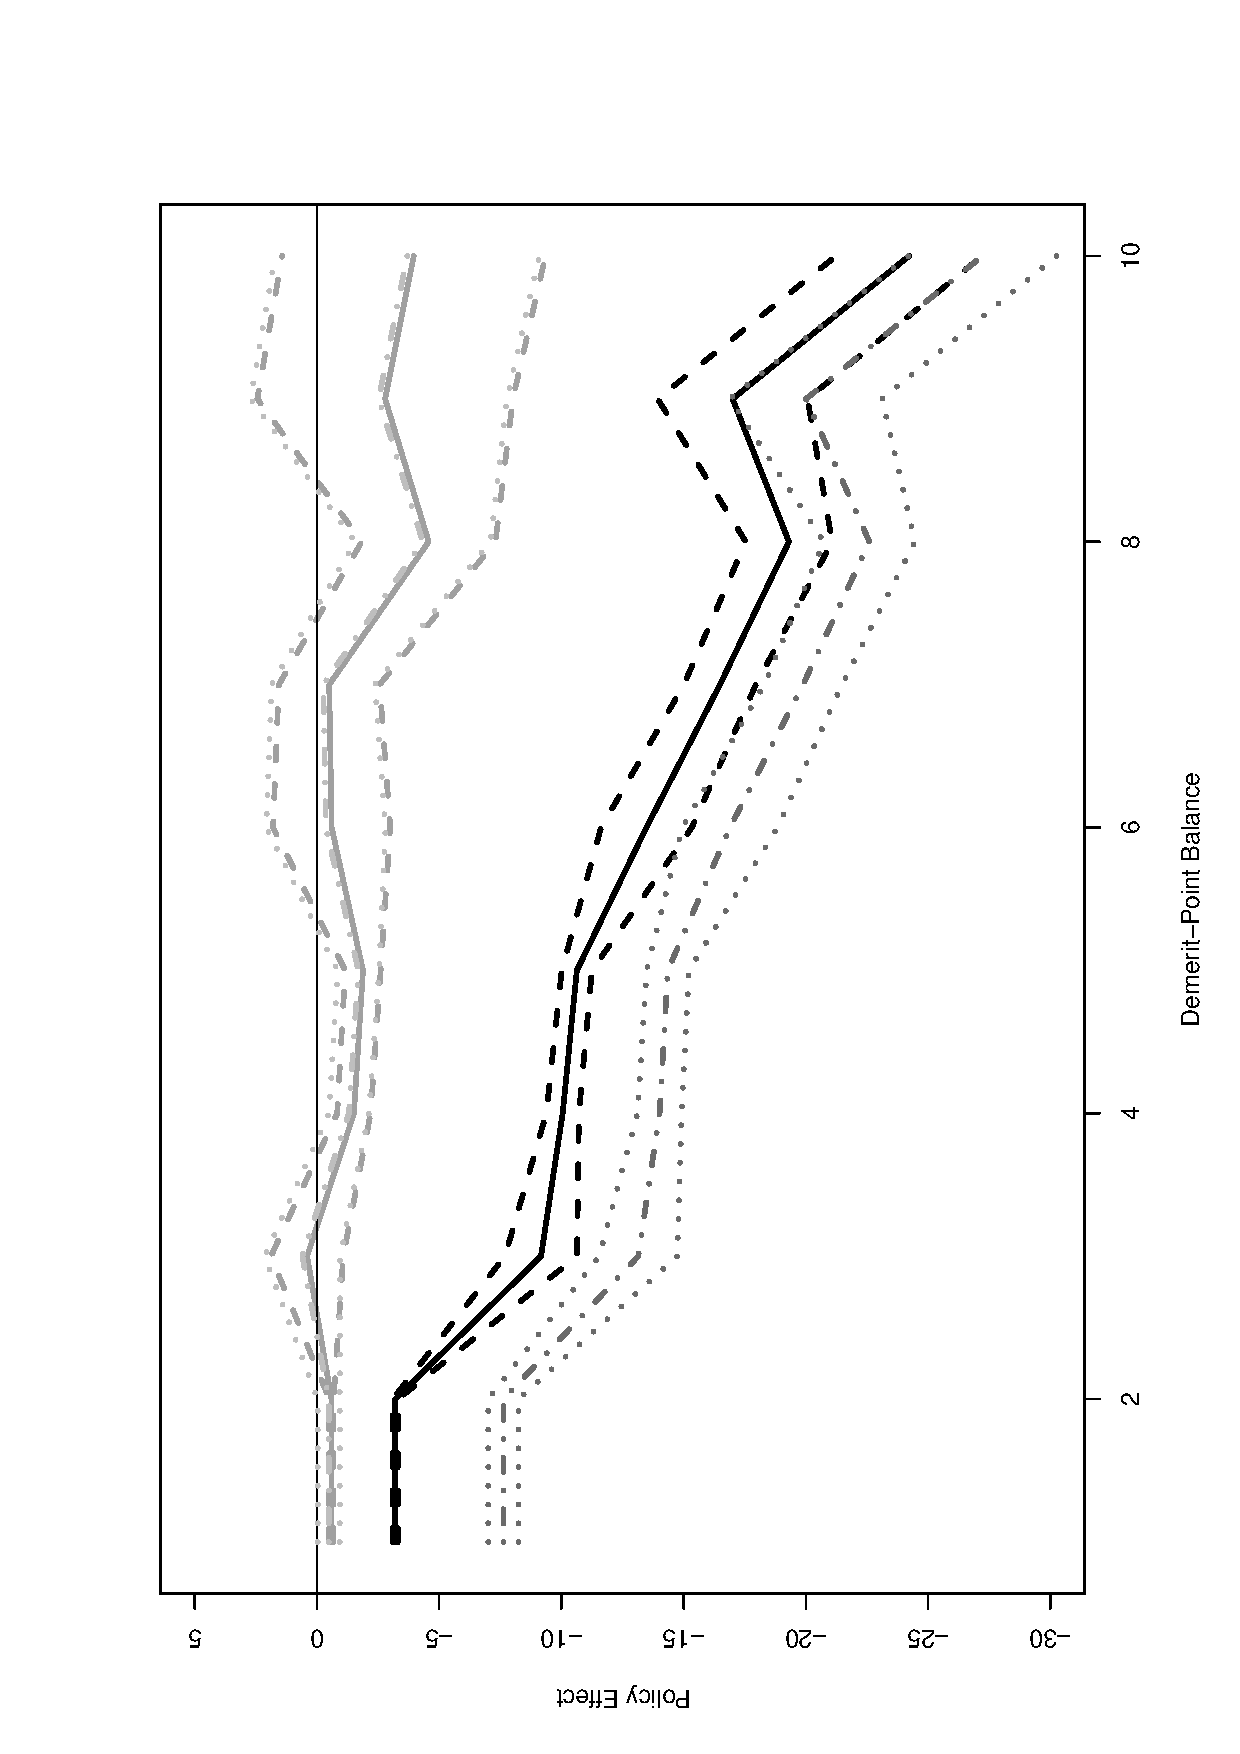
\includegraphics[width=0.8\textwidth, angle =270]{Figure3}
\caption{Policy change and demerit-point group interactions \\
The policy effects for male drivers are shown in black and charcoal
and those for females are shown in grey and light grey.
The darker solid lines show the overall policy effect without an age interaction,
with 95\% confidence intervals shown with dashed lines.
The dashed-and-dotted lines in lighter shades show the policy effect 
for drivers aged 20 to 24
in grey for female drivers and charcoal for male drivers,
with the dotted lines representing the 95\% confidence interval.
Estimates were obtained with the linear probability model
and heteroskedasticity-robust standard errors were calculated 
and, in the case of the model with the age group policy interaction,
using a quadratic form on the covariance matrix to account for the covariance of the
20-24 age group policy effect and the effect for the benchmark age group.
Drivers with ten demerit points or more are all contained in the 10-point category.
}\label{fig:points_fig_with_age_int}
\end{figure}


%%%%%%%%%%%%%%%%%%%%%%%%%%%%%%%%%%%%%%%%

\section{Concerns of Validity}
\label{sec:Validity}


\subsection{Alternative explanations for the downturn in tickets}

To examine the possibility that these results are driven by a secular trend, 
we repeat the regression specified in 
Section \ref{sec:Empirical_all} 
by splitting the pre-period in half. 
Because of the very heterogeneous effects by gender, 
we perform two sets of placebo checks using the regression specification from 
Section \ref{sec:Empirical_all}, 
one for males and one for females. 
The results of this analysis are displayed in 
Table \ref{tab:seas_Logit_vs_LPMx100K_placebo_regs}. 


\begin{table}% [ht] 
\centering 
\begin{tabular}{l r r r r l r r l} 

\hline 
 
 & \multicolumn{5}{c}{Logistic Regression}  & \multicolumn{3}{c}{Linear Probability Model} \\ 

 \cmidrule(lr){2-6}\cmidrule(lr){7-9} 
 & \multicolumn{2}{c}{Marginal Effects} & Estimate & Standard & Sig. & Estimate & Standard & Sig. \\ 

 \cmidrule(lr){2-3} 
 &   AME &  MER  &          &  Error   &      &          &  Error   &     \\ 

\hline 
 
\multicolumn{8}{l}{\textbf{Male Drivers} (2,618,869,407 observations)} \\ 

\hline
\multicolumn{8}{l}{Model without age-policy interaction: } \\ 
Policy                   &  -0.1306        &  -0.5478       &  -0.0024        &  0.0017       &            &  -0.2109        &  0.0905       &            \\ 
\hline
\multicolumn{8}{l}{Model with age-policy interaction: } \\ 
Policy                   &  -1.0812        &  -4.1848       &  -0.0572        &  0.0540       &            &  -1.8092        &  1.0215       &            \\ 
Age 16-19 * policy   &  -1.1446        &  -2.6473       &  -0.0106        &  0.0545       &            &  -2.9360        &  1.3097       &            \\ 
Age 20-24 * policy   &  2.0266        &  4.5628       &  0.0204        &  0.0542       &            &  -0.1000        &  1.1226       &            \\ 
Age 25-34 * policy   &  3.2514        &  8.7684       &  0.0457        &  0.0542       &            &  1.3441        &  1.0507       &            \\ 
Age 35-44 * policy   &  2.8733        &  8.4706       &  0.0496        &  0.0542       &            &  1.2368        &  1.0420       &            \\ 
Age 45-54 * policy   &  3.4577        &  10.9720       &  0.0698        &  0.0542       &            &  1.9795        &  1.0375       &            \\ 
Age 55-64 * policy   &  3.5248        &  12.0052       &  0.0879        &  0.0543       &            &  2.3344        &  1.0386       &            \\ 
Age 65+ * policy   &  3.3942        &  12.9623       &  0.1316        &  0.0545       &            &  2.7337        &  1.0342       &            \\ 

\hline 

\multicolumn{8}{l}{\textbf{Female Drivers} (2,109,880,955  observations)} \\ 

\hline
\multicolumn{8}{l}{Model without age-policy interaction: } \\ 
Policy                   &  -0.1543        &  -0.8795       &  -0.0059        &  0.0027       &            &  -0.1803        &  0.0706       &            \\ 
\hline
\multicolumn{8}{l}{Model with age-policy interaction: } \\ 
Policy                   &  0.8415        &  4.3695       &  0.1696        &  0.1874       &            &  0.6983        &  0.9249       &            \\ 
Age 16-19 * policy   &  -6.8789        &  -26.4519       &  -0.1940        &  0.1879       &            &  -1.1349        &  1.0789       &            \\ 
Age 20-24 * policy   &  -6.4219        &  -23.3417       &  -0.1686        &  0.1875       &            &  -0.0914        &  0.9821       &            \\ 
Age 25-34 * policy   &  -5.7121        &  -22.0027       &  -0.1848        &  0.1875       &            &  -1.0372        &  0.9438       &            \\ 
Age 35-44 * policy   &  -5.4912        &  -21.6223       &  -0.1970        &  0.1875       &            &  -1.4878        &  0.9396       &            \\ 
Age 45-54 * policy   &  -3.7063        &  -15.7414       &  -0.1681        &  0.1875       &            &  -0.8437        &  0.9355       &            \\ 
Age 55-64 * policy   &  -2.4244        &  -11.0054       &  -0.1496        &  0.1876       &            &  -0.6454        &  0.9358       &            \\ 
Age 65+ * policy   &  -1.0624        &  -5.1866       &  -0.1028        &  0.1878       &            &  -0.3173        &  0.9345       &            \\ 

\hline 

\end{tabular} 
\caption{Placebo regressions for all offences} 
For each regression, the dependent variable is an indicator that a driver has committed  
any offence on a particular day.  
All regressions contain age category and demerit point category controls, 
as well as monthly and weekday indicator variables. 
The baseline age category comprises drivers under the age of 16. 
The heading ``Sig.'' is an abbreviation for statistical significance, with 
the symbol * denoting statistical significance at the 0.1\% level 
and ** the 0.001\% level. 
Marginal effects, as well as linear probability model coefficients and standard errors, are  
multiplied by 100,000.  
The linear probability model uses heteroskedasticity-robust standard errors. 
\label{tab:seas_Logit_vs_LPMx100K_placebo_regs} 
\end{table} 
 


The regression results show no statistical evidence of pre-trends, 
and none of the coefficients of interest are precisely estimated. 
Moreover, the magnitude of the coefficients in both placebo regressions 
for the model without age-policy interactions are very similar 
and are far smaller than their counterparts in the real regressions; 
we argue that this is evidence of precisely estimated zeros 
given their magnitude and small standard errors.%
\footnote{% 
Even with the very large sample employed in this analysis, 
unless the effect is exactly zero in the population, 
a non-zero standard error and coefficient estimate will be still be produced. 
For a discussion on precise zeros, see 
\citet{penney2013}. 
}
%
If there were a secular trend in the pre-period driving the results of the main regressions, 
the male coefficient would have a substantially larger magnitude than the female coefficient, 
but this is not the case. 
In the set of regressions containing the age category dummies interacted with the policy variable, 
none of the interactions are statistically significant, and there is no pattern among the coefficients either.
This result contrasts with the coefficients on the age interactions for males 
in the main regression in which we observe a clear pattern: 
the effect is similar from ages 16 to 25, and then slowly declines with age. 
Overall, we do not find any convincing evidence that the effects found in the 
real main regression are an artifact of something other than the excessive speeding laws.


An alternative explanation is the idea that police leniency may have changed as a result of the law; 
we examine this possibility here. 
The introduction of additional penalties for excessive speeding may 
motivate police officers to note tickets as lesser speeding violations. 
For example, excessive speeding in zones with a limit of 60km/h 
could be marked down to a 3-point ticket, 
while excessive speeding in zones with higher limits could be reduced to a 5-point ticket. 
Three arguments speak against this possibility. 
First, police officers could behave in this fashion to avoid appearing in court 
in case the driver contests the charges.  
In Quebec, however, police officers are not required to appear in traffic court.%
\footnote{% 
See the following website (in French) for details: \texttt{https://educaloi.qc.ca/capsules/la-contestation-dune-contravention/} (Accessed July 18, 2020).}  
%
Second, a police officer aiming to be lenient would reduce the speed on a ticket 
to a level where the excessive speeding provisions would not take effect. 
% 
However, according to 
Table \ref{tab:seas_Logit_vs_LPMx100K_regs_by_points}, 
the incidence of tickets for men decreases for every category above 1 point, 
while for women it decreases for every category above 2 points. 
In other words, the categories to which the tickets would be marked down (3-point or 5-point tickets) still saw decreases.%
\footnote{% 
Note that there are no speeding violations worth 4 points under the Quebec highway safety code, and that 4-point tickets are much less common than 3-point or 5-point tickets; see 
Table \ref{tab:point_freq}.
}
% 
Finally, the overall number of tickets per driver-day still decreased (the extensive margin), 
and leniency against the provisions of the excessive speeding law 
would only affect the intensive margin of demerit points. 
We conclude it is very unlikely that a change in police leniency could be driving the results.


\begin{table}% [ht] 
\centering 
\begin{tabular}{l r r r r l r r l} 

\hline 
 
 & \multicolumn{5}{c}{Logistic Regression}  & \multicolumn{3}{c}{Linear Probability Model} \\ 

 \cmidrule(lr){2-6}\cmidrule(lr){7-9} 
 & \multicolumn{2}{c}{Marginal Effects} & Estimate & Standard & Sig. & Estimate & Standard & Sig. \\ 

 \cmidrule(lr){2-3} 
 &   AME & MER &          &  Error   &      &          &  Error   &     \\ 

\hline 
 
\multicolumn{7}{l}{\textbf{Male Drivers} (5,335,033,221 observations)} \\ 

Policy Indicator          &  -4.0366        &  -16.4792       &  -0.0762        &  0.0015       &   **       &  -4.1859        &  0.0763       &   **       \\ 
Month 1                         &  9.9449        &  38.5317       &  0.1483        &  0.0047       &   **       &  8.6823        &  0.2761       &   **       \\ 
Month 2                         &  7.2862        &  27.2675       &  0.1110        &  0.0046       &   **       &  6.6386        &  0.2726       &   **       \\ 
Month 3                         &  2.2160        &  8.3591       &  0.0380        &  0.0048       &   **       &  2.2264        &  0.2683       &   **       \\ 
Month 4                         &  -4.7201        &  -17.3888       &  -0.0965        &  0.0049       &   **       &  -5.0416        &  0.2534       &   **       \\ 
Month 5                         &  -4.1329        &  -17.4499       &  -0.0969        &  0.0052       &   **       &  -4.5641        &  0.2379       &   **       \\ 
Month 6                         &  -6.4410        &  -20.9716       &  -0.1206        &  0.0047       &   **       &  -6.9509        &  0.2708       &   **       \\ 
Month 7                         &  -4.2653        &  -14.4849       &  -0.0782        &  0.0046       &   **       &  -4.4353        &  0.2648       &   **       \\ 
Month 8                         &  -6.3291        &  -22.5706       &  -0.1320        &  0.0049       &   **       &  -7.3088        &  0.2584       &   **       \\ 
Month 9                         &  -4.9332        &  -35.9259       &  -0.2503        &  0.0071       &   **       &  -6.6876        &  0.1737       &   **       \\ 
Month 10                        &  -10.5940        &  -44.5275       &  -0.3699        &  0.0057       &   **       &  -15.3145        &  0.2167       &   **       \\ 
Month 11                        &  -6.2712        &  -23.1921       &  -0.1366        &  0.0051       &   **       &  -7.2667        &  0.2609       &   **       \\ 
Month 12                        &  -2.8571        &  -10.5662       &  -0.0551        &  0.0047       &   **       &  -3.1070        &  0.2560       &   **       \\ 

\hline 

\multicolumn{7}{l}{\textbf{Female Drivers} (4,340,212,273 observations)} \\ 

Policy Indicator          &  0.8179        &  4.6888       &  0.0310        &  0.0022       &   **       &  0.8391        &  0.0611       &   **       \\ 
Month 1                         &  3.7539        &  19.1217       &  0.1063        &  0.0070       &   **       &  3.5263        &  0.2238       &   **       \\ 
Month 2                         &  2.1374        &  10.6644       &  0.0632        &  0.0069       &   **       &  2.2000        &  0.2191       &   **       \\ 
Month 3                         &  -0.4495        &  -2.3531       &  -0.0157        &  0.0074       &            &  -0.3857        &  0.2112       &            \\ 
Month 4                         &  -3.4773        &  -18.6622       &  -0.1527        &  0.0078       &   **       &  -4.0417        &  0.1945       &   **       \\ 
Month 5                         &  -3.2337        &  -19.8371       &  -0.1654        &  0.0083       &   **       &  -3.9171        &  0.1824       &   **       \\ 
Month 6                         &  -4.5281        &  -19.8371       &  -0.1654        &  0.0071       &   **       &  -4.8207        &  0.2167       &   **       \\ 
Month 7                         &  -3.8277        &  -17.3447       &  -0.1390        &  0.0071       &   **       &  -3.9811        &  0.2116       &   **       \\ 
Month 8                         &  -4.5030        &  -21.4857       &  -0.1842        &  0.0074       &   **       &  -5.3036        &  0.2072       &   **       \\ 
Month 9                         &  -2.9968        &  -32.3390       &  -0.3584        &  0.0117       &   **       &  -5.3165        &  0.1302       &   **       \\ 
Month 10                        &  -6.0362        &  -37.1693       &  -0.5268        &  0.0095       &   **       &  -10.3117        &  0.1611       &   **       \\ 
Month 11                        &  -4.3594        &  -22.6167       &  -0.1978        &  0.0080       &   **       &  -5.2484        &  0.2036       &   **       \\ 
Month 12                        &  -2.1026        &  -10.5533       &  -0.0772        &  0.0072       &   **       &  -2.1935        &  0.2059       &   **       \\ 

\hline 

\end{tabular} 
\caption{Regressions with indicators for month since policy change} 
For each regression, the dependent variable is an indicator that a driver has committed  
any offence on a particular day.  
All regressions contain age category and demerit point category controls, 
as well as monthly and weekday indicator variables. 
The baseline age category comprises drivers under the age of 16. 
The heading ``Sig.'' is an abbreviation for statistical significance, with 
the symbol * denoting statistical significance at the 0.1\% level 
and ** the 0.001\% level. 
Marginal effects, as well as linear probability model coefficients and standard errors, are  
multiplied by 100,000.  
The linear probability model uses heteroskedasticity-robust standard errors. 
\label{tab:seas_Logit_vs_LPMx100K_event_month_regs} 
\end{table} 
 



An increase in police vigilance during the implementation of the policy 
could also have affected the magnitude of the results. 
Indeed, it would have increased the number of tickets written in that period, 
which would result in an underestimation of the effect. 
% 
We investigated this possibility by including separate dummy variables
for the first 12 months after the change in laws. 
These results are shown in 
Table \ref{tab:seas_Logit_vs_LPMx100K_event_month_regs}. 
The variable called ``Policy Indicator'' equals 1 for the entire period after
the law came into effect. 
In each of the subsequent 12 months, the effect of the policy is measured 
as the sum of the ``Policy Indicator'' coefficient 
and the coefficient for the numbered month. 
% 
These monthly policy effects are plotted over the two-year period 
after the policy change in Figure \ref{fig:event_study}.
% 
For male drivers, the probability of obtaining any ticket increased by 
$0.00450$ and $0.00245$ percentage points in the first two months of the policy
but decreased by the third month. 
The program had maximum effectiveness over the last half of 2008, 
with a decrease of $0.00729$ percentage points in the twelfth month,
not far from the overall policy effect of $0.00597$ in 
Table \ref{tab:seas_Logit_vs_LPMx100K_regs}. 
% 
For female drivers, the pattern was similar, except that the magnitude 
of the decline was smaller and the effect in the second year was a
small increase in magnitude. 
% 
Together, this suggests some combination of an increase in police vigilance 
and a learning curve over the course of a year. 

\begin{figure}
\centering
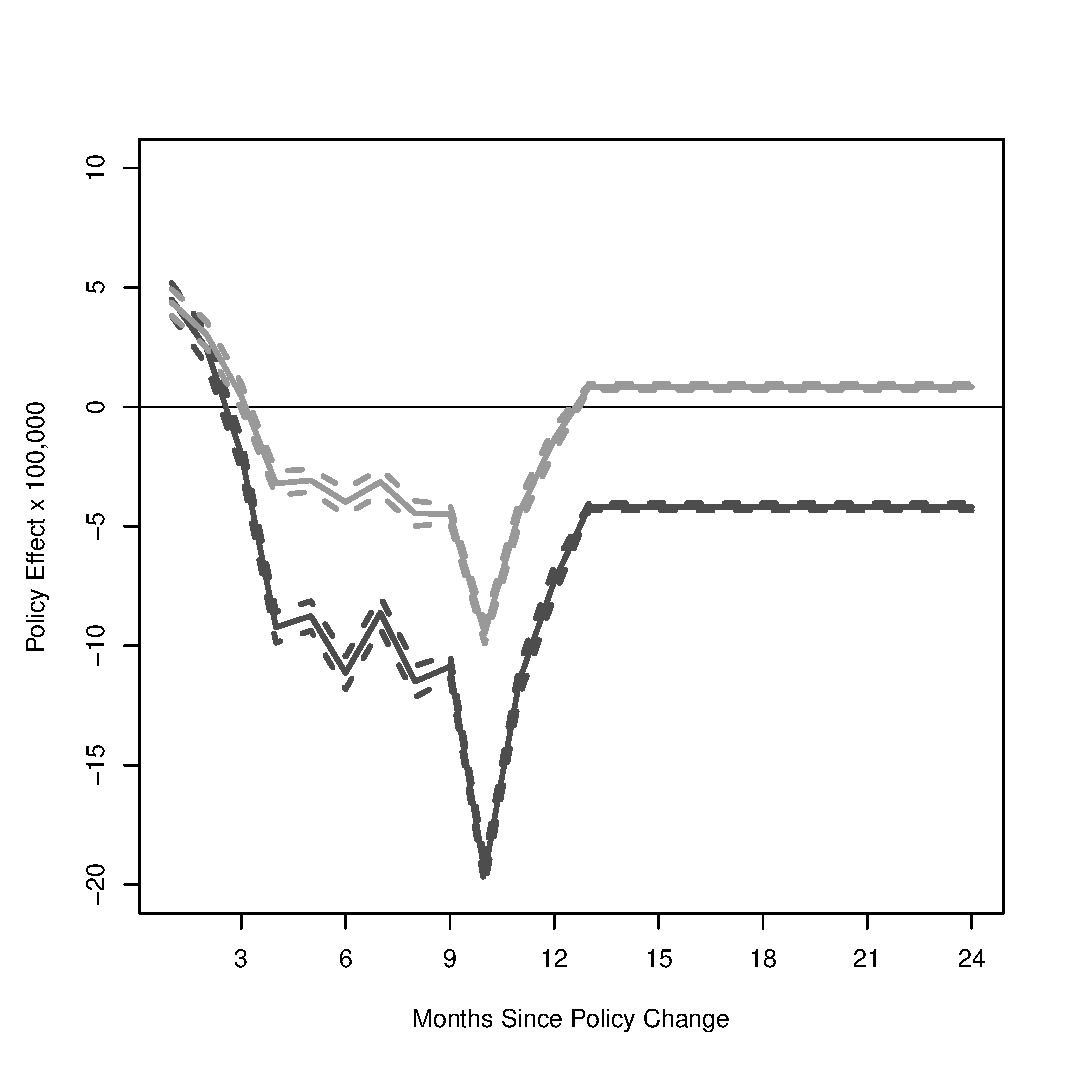
\includegraphics[width=0.8\textwidth]{Figure4}
\caption{Monthly pattern of the policy effects \\
The points along the path reflect the net effect measured by 
the coefficients for the ``Policy Indicator'' 
and the corresponding ``Month'' indicator, 
shown in Table \ref{tab:seas_Logit_vs_LPMx100K_event_month_regs}, 
multiplied by 100,000. 
The black lines represent the effects for males 
and the grey lines those for females. 
The dashed lines are 95\% confidence bands. 
}\label{fig:event_study}
\end{figure}



During about the last third of the sample period after the policy change, 
the province of Quebec introduced a photo radar pilot. 
It started issuing tickets for speeding on August 19, 2009. 
We do not believe this had a substantial effect on driver behaviour for several reasons. 
First, the number of photo radar machines was very small: 
there were 15 in the entire province of Quebec, 
which had a population of approximately 8 million people at the time.%
\footnote{% 
Of these 15, 6 were for speeding, 6 were for red light violations, and 3 were mobile 
\citep{bisson2020}.
}  
%
Second, during the pilot, 
the photo radar machines were placed in plain sight, 
and warning signs were placed ahead of them to clearly alert drivers of their location.

One last consideration is that, in April 2008, 
the Quebec government also introduced new legislation 
banning the use of handheld mobile devices while driving. 
This new violation associated with 3 demerit points could have 
increased the number of violations in the dataset. 
In 2008, there were 18,254 violations for this charge and 48,835 in 2009 
% 
\citep[table 1.3]{SAAQ2010}.
%  
Despite the introduction of these new violations, 
we still observe a decrease in the total number of violations, 
suggesting our results could be underestimating the real impact of the excessive speeding laws.



\subsection{Statistical properties}

For our empirical analysis, we estimated regressions using
both the linear probability model
and logistic regression; both models have limitations
which we address here. 

Concerns may be raised about the mathematical properties of estimates 
derived from the use of linear probability models. 
For example, 
\citet{horraceoaxaca2006}
claim that predicted probabilities outside of the $[0,1]$ interval 
indicate bias and inconsistency of the linear probability model regression estimates. 
For all regressions conducted in our paper, 
no predicted probabilities fall outside of this interval, 
assuaging this concern. 
Furthermore, the absence of negative predictions is not a product of chance: 
because the explanatory variables in our regressions are all categorical variables, 
the predictions are essentially proportions, 
rather than linear predictions from continuous variables. 
This helps to mitigate the usual criticism of the linear probability model. 

We also estimated a model with driver-specific fixed effects
to account for the possibility that the tendency to get tickets
is not independent between drivers within the same category. 
To facilitate the calculation, we aggregated the data across the time dimension
rather than across drivers
to achieve the same degree of data compression as in the regressions reported above.
We augmented these estimates with cluster-robust standard error estimates 
by clustering on the individual drivers. 
For our purposes, this model has severe limitations. 
First, the fixed effects annihilate the age and gender categories, 
which we found were strongly related to driving behaviour
and worth analyzing in a model. 
Second, and more importantly, 
the remaining variation in our dataset comprises 
only the demerit-point balance indicators and the policy indicator. 
Although still of interest, including demerit-point balances is problematic because 
this variable is a moving average of a variable closely related to the dependent variable:
the number of demerit points for a ticket instead of the indicator for a ticket. 
Still, we found a negative policy effect that was decreasing 
in the current demerit-point balance;
however, the estimates were orders of magnitude larger 
than those recorded in the models without fixed effects. 
This finding is explained by the bias introduced by the direct relationship between the demerit-point balance and the dependent variable, 
which we confirmed with simulation evidence. 


Another issue is the relative rarity of the events 
(the driver-days where the dependent variable is equal to 1 rather than 0). 
\citet{kingzheng2001}
show that rare events cause estimated probabilities to be biased downwards for logit estimation 
(in the case where ones are rare relative to zeros). 
The level of the rare events bias is a function of 
the frequency of events relative to the total sample size: 
for example, a sample size of 1,000 with 2 events (0.2\% of the sample) 
may suffer from rare events bias, 
but a sample size of 100,000 with 200 events (also 0.2\%) may not. 
To examine whether rare events bias potentially exists in our analysis, 
we conduct a Monte Carlo experiment as follows. 
We set up a simulation using an effect size that is similar to the regression involving females but uses a much smaller sample size: 
if rare events bias appears absent, 
it should not be a concern of note in the real regression 
which has a sample 100 times larger. 
The simulation has 1,000 repetitions. 
For each, we generate a dataset with 43,390,582 observations 
where 0.00369\% of observations in the pre-period have an event, 
and 0.004449\% in the post-period. 
The effect size of interest is the difference between these two numbers, which is 0.000759\%. 
The results are as follows. 
We find no statistical evidence of rare events bias: 
the mean effect size of the simulations is also 0.000759\% 
and the estimates are tightly distributed, 
with the 25th percentile being equal to 0.000620\%, 
and the 75th percentile to 0.000889\%. 
Moreover, the statistical power is healthy, 
with 30.1\% of the samples producing statistically significant results 
for the effect size at the 0.001\% level; 
this is despite the simulation using a sample size only one one-hundredth 
that of the sample used in the analysis. 
We conclude that it is unlikely that rare events bias 
is influencing the results in a statistically meaningful fashion.



%%%%%%%%%%%%%%%%%%%%%%%%%%%%%%%%%%%%%%%%

\section{Policy Discussion}
\label{sec:Discussion}

This paper studies the impact of an increase in penalties for speeding 
on the number of tickets issued. 
It is important to study this question to improve the demerit point system 
and thus promote roadway safety. 
Our results provide the following policy implications.

First, we find clear evidence of deterrence from the introduction of the excessive speeding law. 
Increasing the number of points associated with certain violations 
decreased the likelihood of tickets issued for these violations. Moreover, the deterrent effect seems particularly effective for drivers with a large number of points or a history of accumulating demerit points. 
Drivers with a large number of points therefore respond to an increase in the severity of penalties.

Second, young males seem to react particularly strongly to such changes in penalties. 
Our model explains this result by using differences in risk aversion across gender. 
However, the model does not distinguish between different types of punishments 
which usually combine a fine and a number of points: 
the fine represents a short-term punishment, 
while the points increase the likelihood of losing one’s licence in the long-term. 
Our results could show that young males are particularly responsive 
to the threat of losing their licence. 
A policymaker who wants to target young male offenders could choose to use demerit points 
since it seems a particularly salient punishment for this group. 
This result opens the door to a literature on the role of gender in deterrence. 
Males and females may be deterred differently by different types of punishments. 
To our knowledge, this literature is still nascent.

Finally, we document a significant spillover effect 
from the introduction of these new penalties. 
Even though excessive speeding events targeted by the law are relatively rare, 
the law appears to have influenced many drivers. 
Indeed, if the only reactions were from people usually speeding well above the speed limit, 
we would likely not find statistically detectable effects in the overall sample, 
given the low share of tickets for excessive speeding 
(see Table \ref{tab:point_freq}). 
Overall, the legislation decreased the number of violations 
and caused people who habitually drive above the limit to speed less. 
The reason for this spillover effect is somewhat puzzling. 
We speculate that the excessive speeding law made people more aware of speeding penalties in general. 
Since drivers do not always pay close attention to how fast they are driving, 
the threat of more severe penalties may have increased their 
awareness for their speed in more mundane circumstances.


%%%%%%%%%%%%%%%%%%%%%%%%%%%%%%%%%%%%%%%%

\vfill
\eject

%%%%%%%%%%%%%%%%%%%%%%%%%%%%%%%%%%%%%%%%

\clearpage

\bibliographystyle{cjebibstyle}

\bibliography{References}

\vfill
\eject

%%%%%%%%%%%%%%%%%%%%%%%%%%%%%%%%%%%%%%%%
\end{document}
%%%%%%%%%%%%%%%%%%%%%%%%%%%%%%%%%%%%%%%%
